\chapter{Proverb 29}

\begin{figure}
  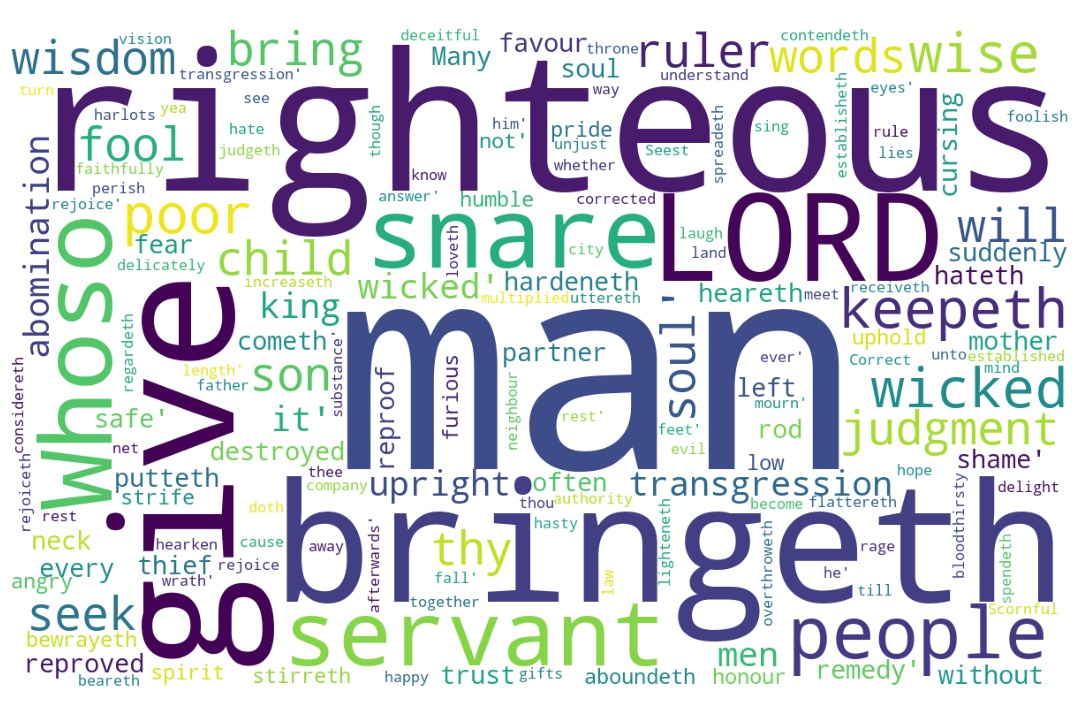
\includegraphics[width=\linewidth]{20OT-Proverbs/Proverb29-WordCloud.jpg}
  \caption{Proverb 29 Word Cloud}
  \label{fig:Proverb 29 word Cloud}
\end{figure}

\marginpar{\scriptsize \centering \fcolorbox{bone}{lime}{\textbf{MISSING WITHOUT WISDOM}}\\ (Proverb 29:1--27) 
\begin{compactenum}[I.][8]
    \item No \textbf{Remedy} \index[scripture]{Proverbs!Pro 29:01}(Pro 29:1) 
    \item No \textbf{Remorse} \index[scripture]{Proverbs!Pro 29:02}(Pro 29:2) 
    \item No \textbf{Rejoicing} \index[scripture]{Proverbs!Pro 29:06}(Pro 29:6) 
    \item No \textbf{Regard} \index[scripture]{Proverbs!Pro 29:07}(Pro 29:7) 
    \item No \textbf{Rest} \index[scripture]{Proverbs!Pro 29:09}(Pro 29:9) 
    \item No \textbf{Reproof} \index[scripture]{Proverbs!Pro 29:15}(Pro 29:15) 
    \item No \textbf{Restraint} \index[scripture]{Proverbs!Pro 29:16}(Pro 29:16) 
\end{compactenum} }

\footnote{\textcolor[cmyk]{0.99998,1,0,0}{\hyperlink{TOC}{Return to end of Table of Contents.}}}\footnote{\href{https://www.audioverse.org/english/audiobibles/books/ENGKJV/O/Prov/1}{\textcolor[cmyk]{0.99998,1,0,0}{Proverbs Audio}}}\textcolor[cmyk]{0.99998,1,0,0}{He, that being often reproved hardeneth \fcolorbox{bone}{bone}{his} neck, shall suddenly be destroyed, and that without \fcolorbox{bone}{lime}{remedy}.}
[2] \textcolor[cmyk]{0.99998,1,0,0}{When the righteous are in authority, the people rejoice: \fcolorbox{bone}{bone}{but} when the wicked beareth rule, the people \fcolorbox{bone}{lime}{mourn}.}
[3] \textcolor[cmyk]{0.99998,1,0,0}{Whoso loveth wisdom rejoiceth \fcolorbox{bone}{bone}{his} father: \fcolorbox{bone}{bone}{but} he that keepeth company with harlots spendeth \emph{his} substance.}
[4] \textcolor[cmyk]{0.99998,1,0,0}{The king by judgment establisheth the land: \fcolorbox{bone}{bone}{but} he that receiveth gifts overthroweth it.}
[5] \textcolor[cmyk]{0.99998,1,0,0}{A man that flattereth \fcolorbox{bone}{bone}{his} neighbour spreadeth a net for \fcolorbox{bone}{bone}{his} feet.}
[6] \textcolor[cmyk]{0.99998,1,0,0}{In the transgression of an evil man \emph{there} \emph{is} a snare: \fcolorbox{bone}{bone}{but} the righteous doth sing and \fcolorbox{bone}{lime}{rejoice}.}
[7] \textcolor[cmyk]{0.99998,1,0,0}{The righteous considereth the cause of the poor: \emph{but} the wicked \fcolorbox{bone}{lime}{regardeth} not to know \emph{it}.}
[8] \textcolor[cmyk]{0.99998,1,0,0}{Scornful men bring a city into a snare: \fcolorbox{bone}{bone}{but} wise \emph{men} turn away wrath.}
[9] \textcolor[cmyk]{0.99998,1,0,0}{\emph{If} a wise man contendeth with a foolish man, whether he rage or laugh, \emph{there} \emph{is} no \fcolorbox{bone}{lime}{rest}.}
[10] \textcolor[cmyk]{0.99998,1,0,0}{The bloodthirsty hate the upright: \fcolorbox{bone}{bone}{but} the just seek \fcolorbox{bone}{bone}{his} soul.}
[11] \textcolor[cmyk]{0.99998,1,0,0}{A fool uttereth all \fcolorbox{bone}{bone}{his} mind: \fcolorbox{bone}{bone}{but} a wise \emph{man} keepeth it in till afterwards.}
[12] \textcolor[cmyk]{0.99998,1,0,0}{If a ruler hearken to lies, all \fcolorbox{bone}{bone}{his} servants \emph{are} wicked.}
[13] \textcolor[cmyk]{0.99998,1,0,0}{The poor and the deceitful man meet together: the LORD lighteneth both their eyes.}
[14] \textcolor[cmyk]{0.99998,1,0,0}{The king that faithfully judgeth the poor, \fcolorbox{bone}{bone}{his} throne shall be established for ever.}
[15] \textcolor[cmyk]{0.99998,1,0,0}{The rod and \fcolorbox{bone}{lime}{reproof} give wisdom: \fcolorbox{bone}{bone}{but} a child left \emph{to} \emph{himself} bringeth \fcolorbox{bone}{bone}{his} mother to shame.}
[16] \textcolor[cmyk]{0.99998,1,0,0}{When the wicked are multiplied, \fcolorbox{bone}{lime}{\fcolorbox{bone}{MYGOLD}{transgression} increaseth}: \fcolorbox{bone}{bone}{but} the righteous shall see their fall.}
[17] \textcolor[cmyk]{0.99998,1,0,0}{Correct thy son, and he shall give thee rest; yea, he shall give delight unto thy soul.}
[18] \textcolor[cmyk]{0.99998,1,0,0}{Where \emph{there} \emph{is} no vision, the people perish: \fcolorbox{bone}{bone}{but} he that keepeth the law, happy \emph{is} he.}
[19] \textcolor[cmyk]{0.99998,1,0,0}{A servant will not be corrected by words: for though he understand he will not answer.}
[20] \textcolor[cmyk]{0.99998,1,0,0}{Seest thou a man \emph{that} \emph{is} hasty in \fcolorbox{bone}{bone}{his} words? \emph{there} \emph{is} more hope of a fool than of him.}
[21] \textcolor[cmyk]{0.99998,1,0,0}{He that delicately bringeth up \fcolorbox{bone}{bone}{his} servant from a child shall have him become \emph{his} son at the length.}
[22] \textcolor[cmyk]{0.99998,1,0,0}{An angry man stirreth up strife, and a furious man aboundeth in transgression.}
[23] \textcolor[cmyk]{0.99998,1,0,0}{A man's pride shall bring him low: \fcolorbox{bone}{bone}{but} honour shall uphold the humble in spirit.}
[24] \textcolor[cmyk]{0.99998,1,0,0}{Whoso is partner with a thief hateth \fcolorbox{bone}{bone}{his} own soul: he heareth cursing, and bewrayeth \emph{it} not.}
[25] \textcolor[cmyk]{0.99998,1,0,0}{The fear of man bringeth a snare: \fcolorbox{bone}{bone}{but} whoso putteth \fcolorbox{bone}{bone}{his} trust in the LORD shall be safe.}
[26] \textcolor[cmyk]{0.99998,1,0,0}{Many seek the ruler's favour; \fcolorbox{bone}{bone}{but} \emph{every} man's judgment \emph{cometh} from the LORD.}
[27] \textcolor[cmyk]{0.99998,1,0,0}{An unjust man \emph{is} an abomination to the just: and \emph{he} \emph{that} \emph{is} upright in the way \emph{is} abomination to the wicked.}


